% !TEX root =  master.tex
\graphicspath{ {./img/} }

\chapter{Konzeption - Hardware}\label{Hardware - Konzeption}

\nocite{*}

Für die Umsetzung eines selbstspielenden Klaviers wurden verschiedene technische Überlegungen angestellt.
Die Grundfragen, denen wir bei der Konstruktion begegneten, betrafen die Auswahl und Implementierung der
Aktuatoren, die Methode des Anspielens der Klaviertasten sowie die Signalübertragung des Arduinos.
Im Hinblick auf die Aktuatoren fiel unsere Wahl auf Hubmagneten, die eine präzise Steuerung der Tasten
ermöglichen. Durch ihre Verwendung können die Tasten des Klaviers mit der erforderlichen Geschwindigkeit und
Genauigkeit angespielt werden. \newline
Die Aktuatoren wurden mit den Klaviertasten mittels Seilen verbunden, um die mechanische Integrität des Klaviers
zu erhalten und gleichzeitig eine präzise Steuerung zu gewährleisten.\newline
Die Signalübertragung erfolgte über einen Arduino-Mikrocontroller. Da der Arduino nicht über ausreichend
viele Ausgänge verfügt, um alle Tasten anzusteuern, wurde das Signal mithilfe von Schieberegistern erweitert.
Diese Erweiterung ermöglichte es, alle 88 Tasten des Klaviers anzusteuern, ohne zusätzliche Hardware einsetzen
zu müssen.

\section{Elektronik}\label{Vorgehen - Hardware}


\subsection{Arduino R3}\label{Ansteuerung}
Zur Signalsteuerung wird ein Arduino R3 genutzt.
Es handelt sich dabei um eine Open-Source-Plattform für die Entwicklung von elektronischen Prototypen. Er besteht aus
einem Mikrocontroller-Board, das mit verschiedenen Sensoren, Aktuatoren und anderen elektronischen Komponenten
verbunden werden kann. Der Arduino verfügt über digitale und analoge Ein- und Ausgangspins, die für die Interaktion mit
externen Geräten verwendet werden können. \newline
Der Arduino Uno R3 eignet sich hervorragend zur Ansteuerung der Aktuatoren eines selbstspielenden Klaviers aus
mehreren Gründen. Erstens bietet der Arduino eine benutzerfreundliche Plattform für die Entwicklung und Implementierung
von Steuerungslogik. Die einfache Programmierung mittels der Arduino-IDE ermöglicht es, komplexe Steuerungsalgorithmen
für die Aktuatoren zu erstellen. \newline
Zweitens bietet er PWM (Pulsweitenmodulation) Pins, die im Rahmen des Projekts genutzt wurden.
//TODO: Speicher \newline
//TODO: Vergleich mit anderen Microcontrollern

\subsection{Pulsweitenmodulation (PWM)}\label{PWM}
PWM ist einfach ausgedrückt eine Technik, bei der die Zeitdauer eines digitalen Signals variiert wird, um einen
durchschnittlichen Wert zu erzeugen. Dies ermöglicht es, die Aktuatoren mit verschiedenen Stärken anzusteuern, indem die
Pulsweite des Signals
entsprechend angepasst wird. Dadurch können die Klaviertasten mit unterschiedlichen Intensitäten angespielt werden,
was zu einer realistischeren und dynamischeren Wiedergabe führt.\newline

Eine Digitale Steuerung wird verwendet, um eine Rechteckwelle - ein Signal das zwischen Ein und Aus umgeschaltet wird
- zu erzeugen. Dieses Ein-Aus-Muster kann Spannungen zwischen der vollen Versorgungsspannung (5V) und Aus (0 Volt)
simulieren.
Dabei wird der Anteil der Zeit geändert, den das Signal eingeschaltet ist im Vergleich zur Zeit, die das Signal
ausgeschaltet ist. Die Dauer der Einschaltzeit wird als Pulsweite bezeichnet. Um unterschiedliche analoge Werte zu
erhalten, wird die Pulsweite geändert bzw. moduliert. Wenn dieses Ein-Aus-Muster schnell genug mit einer LED
wiederholt wird, resultiert daraus eine konstante Spannung zwischen 0 und Vcc, die die Helligkeit
der LED steuert. \newline

Auf den Arduino bezogen sieht die Umsetzung eines PWM Signals wie folgt aus:
Ein Taktsignal gelangt in die entsprechende Clock.
Die Clock stellt den entsprechenden PWM-Modus ein. Dabei werden zwei wichtige Werte gesetzt:
Der erste bestimmt, wann das Signal von HIGH auf LOW
umschaltet, während der zweite bestimmt, wann es zurückkommt. Das Verhältnis zwischen HIGH und LOW wird als
Tastverhältnis bezeichnet und bestimmt die Helligkeit unserer LED bzw. die Stärke, mit welcher der Hubmagnet anschlägt.
Je länger die Ausgabe im HIGH-Zustand bleibt, desto schneller erfolgt der Tastenanschlag. \newline

Neben dem Tastverhältnis, also das Verhältnis der Einschaltzeit zur
Periodendauer, welches oft in Prozent ausgedrückt wird, ist auch die Resolution (de: Auflösung) ein variierbarer Parameter.
Die Resolution bezieht sich auf die Anzahl der möglichen diskreten Werte, die das Signal annehmen kann.



\subsection{Vermehrung der Ausgänge}
Es werden 88 Tasten angesteuert. Da ein Arduino keine 88 PWM-Ports besitzt, müssen die Signale über
eine Erweiterung der Ausgänge an die Motoren weitergegeben werden. Dafür gibt es mehrere Möglichkeiten:

\begin{enumerate}
	\item Schieberegister
	\item Motor-Matrix
	\item Demultiplexer
\end{enumerate}

\paragraph{Schieberegister}
Ein Schieberegister ist ein integrierter Schaltkreis, der hier verwendet wird, um die Anzahl der verfügbaren Ausgänge des
Mikrocontrollers zu erweitern. Das gängigste Schieberegister ist das 8-Bit-Schieberegister. \newline

Um 88 Ausgänge mit Hilfe von Schieberegistern von nur 3 PWM-Pins des Arduinos anzusteuern, werden insgesamt 11
Schieberegister benötigt.\newline

Zuerst werden die Datenleitungen (SERIAL IN) aller Schieberegister in Reihe geschaltet. Dies bedeutet, dass das
Ausgangssignal des ersten Schieberegisters mit dem Eingang (SERIAL IN) des nächsten verbunden wird, und so weiter, bis
zum letzten Schieberegister. \newline
Der Arduino sendet Daten seriell über die verbundenen PWM-Pin. Diese Daten werden über ein Schieberegister an
alle Schieberegister weitergegeben. Durch diesen Vorgang werden die Daten parallel über alle Schieberegister gesendet.
\newline
Die Ausgänge der Schieberegister (Q0 bis Q7) werden dann an die entsprechenden Aktuatoren angeschlossen.
Das Signal wird zu einer definierten Clock durch die Schieberegister durchgeschoben. So kann durch Steuerung der Daten,
die an die Schieberegister gesendet werden, kann der Arduino jeden einzelnen Ausgang manipulieren, um die Aktuatoren
entsprechend anzusteuern. \newline
Auf diese Weise kann der Arduino mit Hilfe von Schieberegistern eine größere Anzahl von Ausgängen kontrollieren, als er
direkt verfügbar hat.


\paragraph{Motor-Matrix}
Die Motor-Matrix ist einer LED-Matrix nachgeahmt.
In einer Matrix, werden zwei Reihen an Ports angeschlossen, nach folgendem Muster:
$$
\begin{pmatrix}
	(11) & (12) & (13) & (14) & (15) & (16) & (17) & (18) \\
	(21) & (22) & (23) & (24) & (25) & (26) & (27) & (28) \\
	(31) & (32) & (33) & (34) & (35) & (36) & (37) & (38) \\
	(41) & (42) & (43) & (44) & (45) & (46) & (47) & (48) \\
	(51) & (52) & (53) & (54) & (55) & (56) & (57) & (58) \\
	(61) & (62) & (63) & (64) & (65) & (66) & (67) & (68) \\
	(71) & (72) & (73) & (74) & (75) & (76) & (77) & (78) \\
	(81) & (82) & (83) & (84) & (85) & (86) & (87) & (88)
\end{pmatrix}
$$


Eine LED-Matrix besteht aus einer Anordnung von LEDs in Zeilen und Spalten. Jede LED kann unabhängig von den anderen
ein- oder ausgeschaltet werden. Die Steuerung erfolgt über Multiplexing, bei dem jede Zeile der Matrix nacheinander
aktiviert wird, während die entsprechenden LEDs in den Spalten gleichzeitig eingeschaltet werden. Durch schnelles
Wechseln zwischen den Zeilen (PWM) erscheint es den BetrachterInnen, als ob alle LEDs gleichzeitig leuchten würden,
obwohl sie tatsächlich nacheinander aktiviert werden. \newline

Um das Prinzip einer LED-Matrix auf Aktuatoren zu übertragen, müssen lediglich die LEDs durch die Aktuatoren ersetzt werden.
Durch Steuerung der Zeilen und Spalten dieses Rasters können verschiedene Motoren selektiv
aktiviert werden. Dies ermöglicht eine effiziente Steuerung mehrerer Motoren mit einem begrenzten Satz von
Steuersignalen. \newline

//TODO: Nachteile Matrix


\paragraph{Demultiplexer}
//TODO

\subsection{Transistor}
\subsection{Aktuator}\label{subsec:aktuator}
Test
\subsection{Schaltplan}

\textit{Arduino}

Im Zentrum der Schaltung steht der Mikrocontroller (hier: Arduino Uno R3).
Dieser erhält Daten und Strom über den integrierten USB-Anschluss, welcher mit dem Computer verbunden wird.
Da der Arduino limitierte \nameref{PWM}-fähige Ausgänge bereitstellt, werde Schieberegister (74HC595) verwendet.
Mit jedem \"in Reihe" geschaltetem Schieberegister kann die Anzahl PWM-fähiger Ausgänge um 8 erweitert werden.

\textit{Schieberegister}

Der Arduino wird an fünf Stellen mit dem ersten Schieberegister verbunden:

Arduinoport D2 <-> Serial (SER) Input

Über diese Verbindung werden serielle Daten werden hier bitweise in das Register geschoben.

Arduinoport D3 <-> SHCP (Shift Register Clock Input)

Dieser Pin wird verwendet, um den Takt für das Verschieben der Daten innerhalb des Schieberegisters anzulegen.
Bei jedem Taktimpuls auf diesem Pin wird das Bit am seriellen Dateneingang in das Register verschoben.
Das bedeutet, dass bei jeder steigenden Flanke des Taktsignals das Datenbit, das am Eingang anliegt, in das Schieberegister übernommen und alle vorhandenen Daten um eine Position verschoben werden.

Arduinoport D4 <-> STCP (Storage Register Clock Input)

Nachdem die Daten in das Schieberegister eingelesen wurden, wird dieser Pin verwendet, um die im Schieberegister vorhandenen Daten in das Ausgangsregister zu übertragen.
Ein Taktimpuls auf diesem Pin bewirkt, dass die Daten vom Schieberegister ins Ausgangsregister übernommen werden, sodass alle Ausgänge gleichzeitig aktualisiert werden.
Das ist besonders relevant, da sonst unter Umständen alle Ausgänge von einer Änderung im letzten Schieberegister bedingst wären.

Arduino GND <-> Ground, Output Enable (OE)

Der OE-Pin wird genutzt, um die Ausgänge des Schieberegisters global zu aktivieren oder zu deaktivieren, ohne die Daten selbst zu beeinflussen.
Da das Schieberegister zu keiner Zeit deaktiviert sein soll, wird dieser Pin dauerhaft mit dem GND-Pin verbunden.

Arduino VCC 5V <-> VCC, $\overline{SRCLR}$ (Reset)

Um das Schiebregister mit den benötigten 5V zu betreiben, wird der entsprechende Pin mit dem 5V Output des Arduino verbunden.
Zusätzlich wird der $\overline{ }$ SRCLR Port des Schieberegisters, welcher ein Reset ermöglicht dauerhaft mit 5V verbunden.

Jedes weiteres Schieberegister greift die oben genannten Signale ab.
Der einzige Unterschied befindet sich am Serial (SER) Input Port.
Das Schieberegister an Position i+1 wird mit dem seriellen Output des Schieberegisters an Position i verbunden. ($\forall i = 0,...,10$)

\textit{MOSFET}

Die Hubmagnete werden jeweils mit 24V und mit bis zu 400mA betrieben.
Um einen hohen Stromfluss zu steuern, können Transistoren verwendet werden.
Für hohe Spannungen und schnelle Schaltvorgänge eigenen sich besonders MOSFETs (Metall-Oxid-Halbleiter-Feldeffekttransistor).
Im Folgenden werden speziell n-MOSFETs verwendet, der mit einem Signal zwischen 0V (leitet nicht) und +5V (voll leitend) angesteuert werden kann.

Der folgende Aufbau ist für die insgesamt 88 Ausgänge der 11 Schieberegister identisch, da jeder Ausgang für die Ansteuerung genau eines Motors zuständig ist.

Der GATE-Pin des MOSFETs erhält das Signal, dass die \"Durchlässigkeit" steuert aus einem der Outputs des Schieberegisters.
Der SOURCE-Pin wird mit Ground des gesamten Systems verbunden.
Der DRAIN-Pin wird direkt mit dem entsprechenden Kontakt am Hubmagneten verbunden.

\textit{Hubmagnet}

Um den Stromkreis zu schließen wird der andere Kontakt des Hubmagnetes mit dem +24V verbunden.

\textit{Testen}

Um die Fehlersuche zu erleichtern, werden LEDs in den Schaltplan mit eingebaut.
Diese werden jeweils mit einem entsprechenden $1k\Omega$ parallel zu den Motoren angeschlossen.
So kann anhand der Helligkeit der LED die Intensität abgelesen werden, mit der eine Taste gespielt wird.

//Bild vom Schaltplan

\section{Mechanik}\label{vorgehenHW}

\subsection{Auswahl des Klaviers}

Da sich dieses Projekt nicht auf die theoretische Konzeption beschränkt, muss ein entsprechendes Testobjekt - ein reales Klavier - gefunden werden.
Dieses muss einige Voraussetzungen erfüllen:
	1. Der Preis muss im Rahmen des Budgets liegen
	2. Es muss leicht auseinander zu bauen sein, um die Mechanik zugänglich zu machen
	3. Es muss vollständig sein (alle 88 Tasten)
	4. Es muss stimmbar sein
	5. Der Transport muss einfach durchzuführen sein


\subsection{Ansteuerungskonzept}

//Drücken der ziehen, oben oder unten...
1. Oben
	Klavierhand
	Schiene
	Aufsatz mit 88 oben drüber
2. unten
	ziehen
	drücken

\subsection{Anbringung der Aktuatoren}
Beim Ansteuerungskonzept der Tasten muss auch beachtet werden, wo die Magnete befestigt werden.
Wir haben ein Brett, auf welchem sie befestigt werden. Folgende Bedenken:
1. Wie viel Platzt zwischen Solenoids?-weil Hitze
bsp. weiß unten und schwarz oben, weil die weißen weiter vorne
	-> nicht weil funktionalität vor optik (weil zu eng)
 -> Platz maximieren

2. Wie verbinden ohne dass Angelschnuren und andere Solenoids sich in den weg kommen
(3. spezifischer . in 2 oder 3 Reihen)
Voteil: Hitze
Nachteil: Umlenkung, Verkabelung

4. Umlenkung, damit der ganze Hub verwendet werden kann

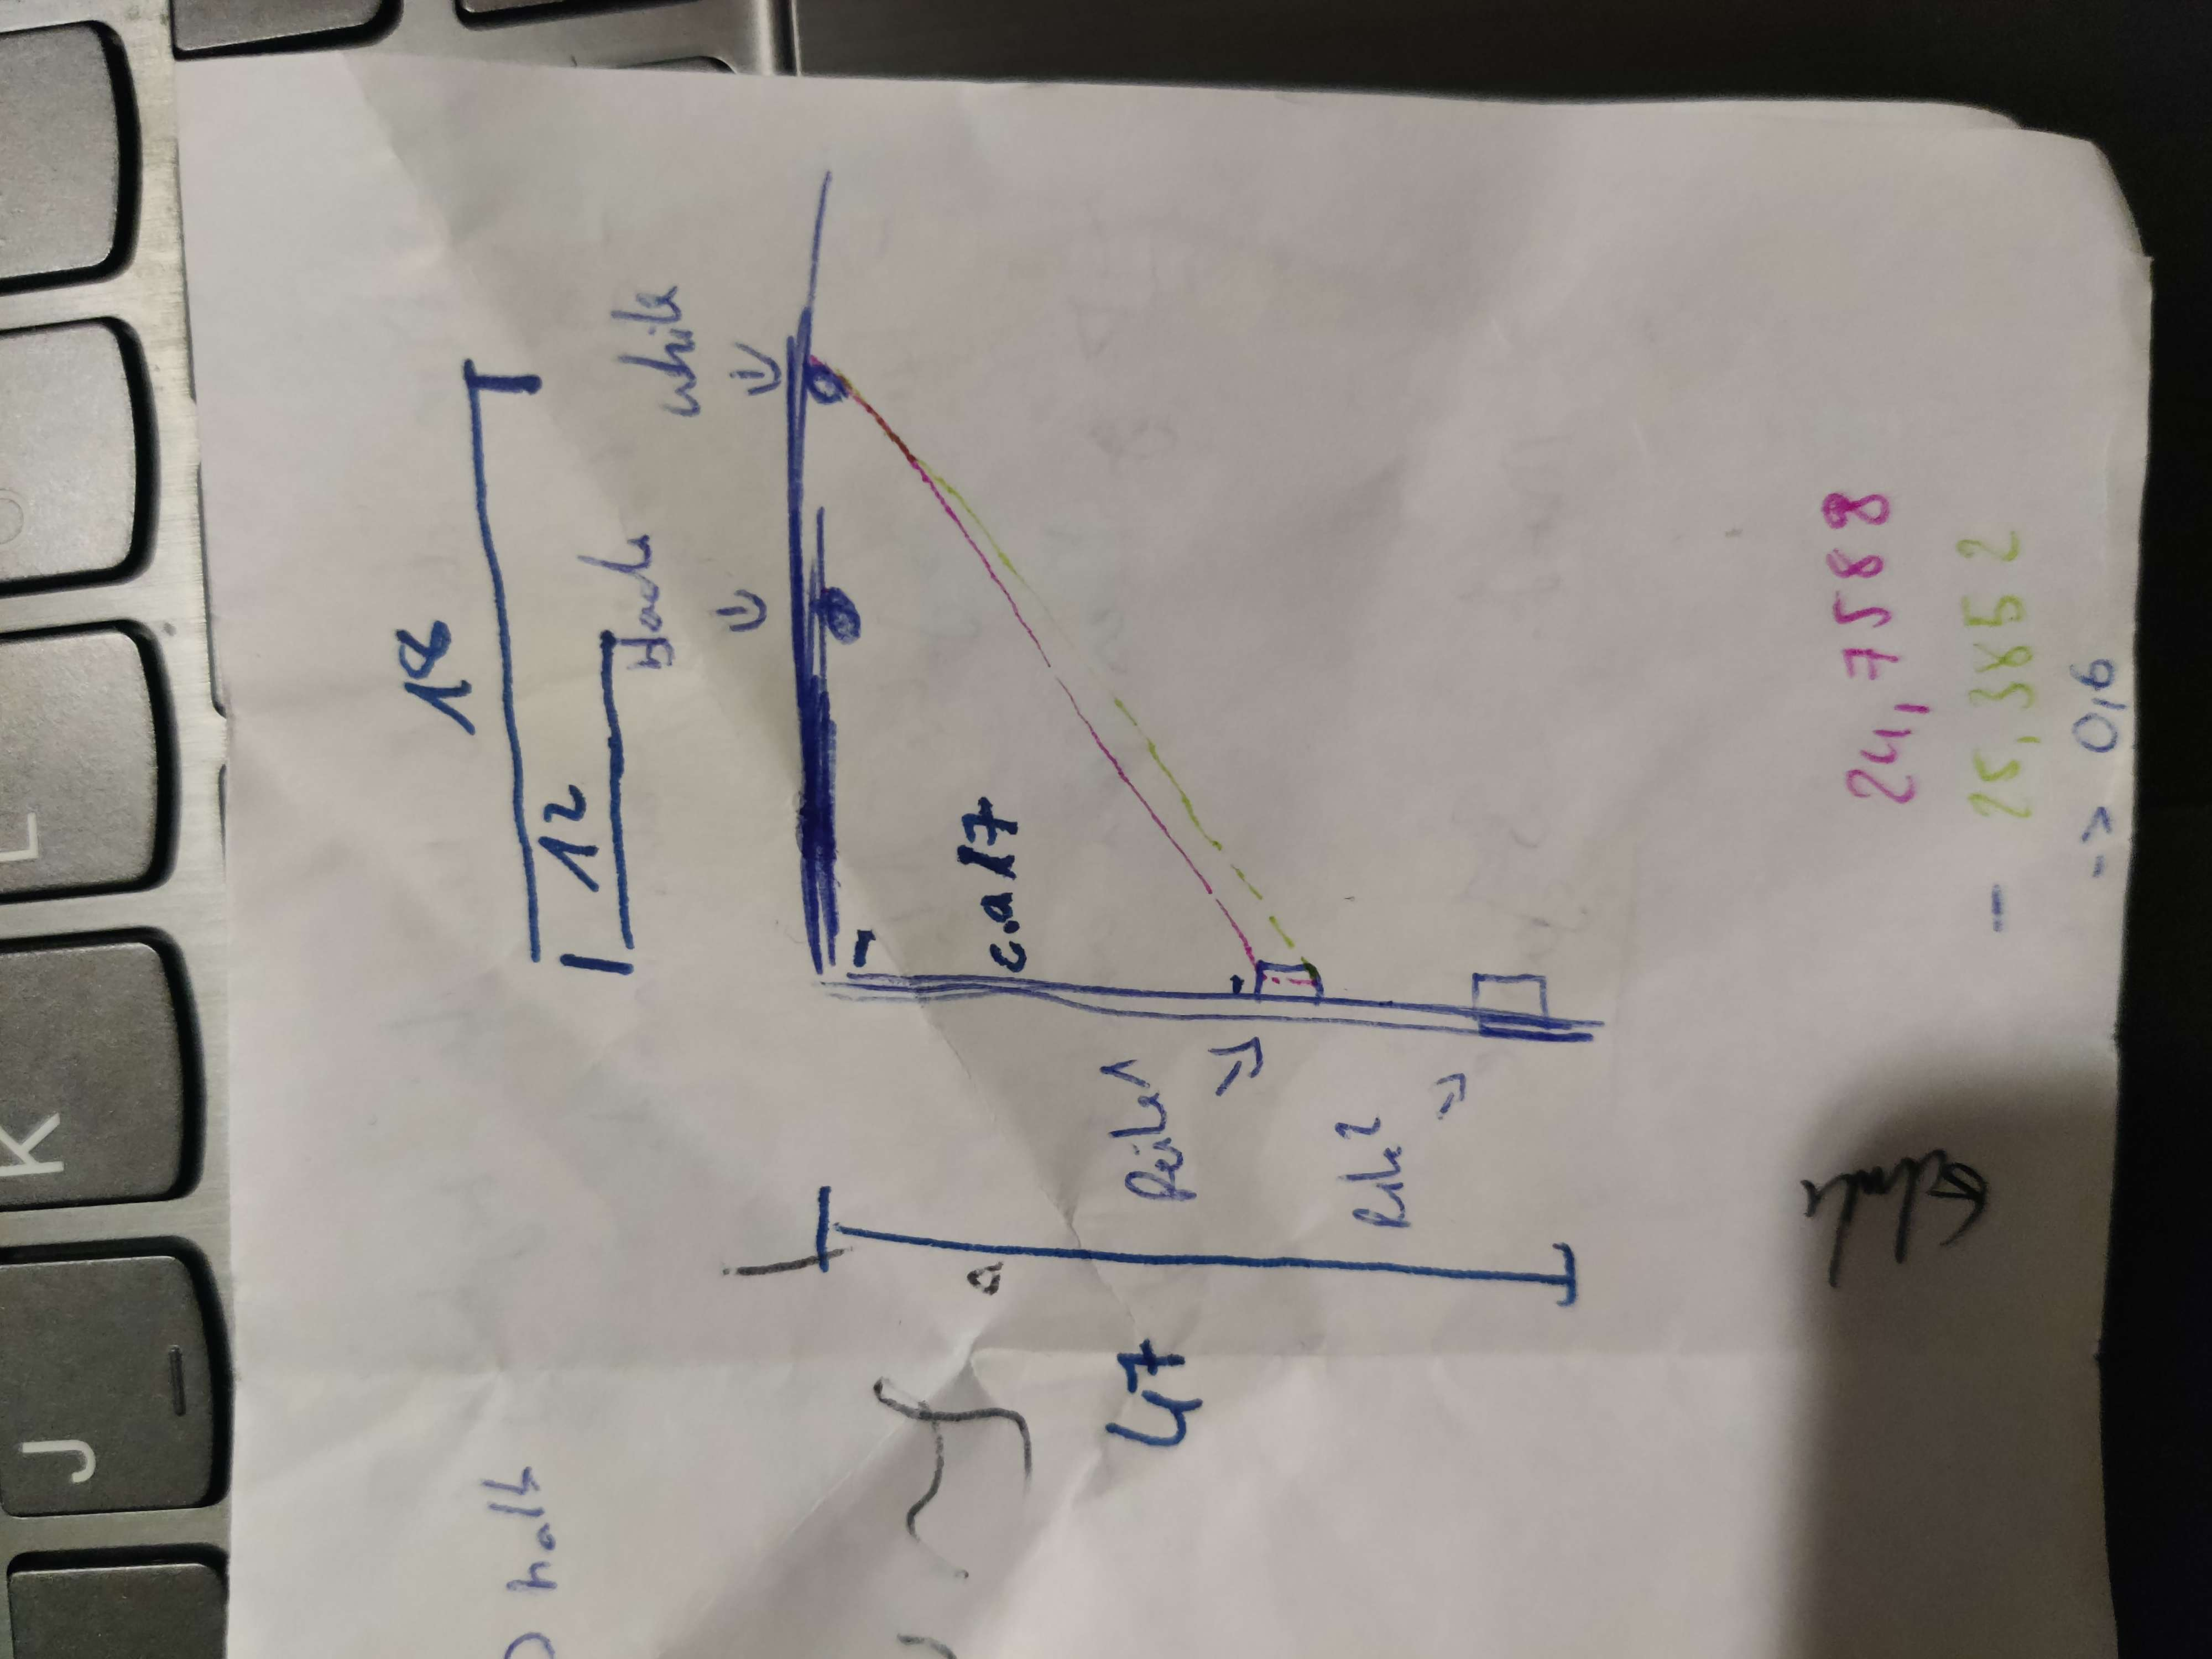
\includegraphics [width=5cm, height=4cm,angle=-90] {img/skizze_Umlenkung}

*Bild wegen Umlenkung

Erklärung geben: Haben Brett mit 67x25cm für 44 Motoren
*Bild von Brett-Sikzze



\subsection{Verbindung Tasten und Hubmagnete}

Es wurde sich dazu entschieden die Tasten durch Ziehen anzusprechen (siehe:\nameref{Ansteuerung}).
Die Grundidee ist, eine Schnur, oder Ähnliches, durch ein waagerechtes Loch in der Taste zu befestigen.
Anschließend wird die Schnur durch ein senkrechtes Loch durch das Holz, worauf die Tasten liegen, in den Fußraum geführt.
Damit der Pianist:in nicht durch Platzmangel eingeschränkt wird, werden die Seile entlang der Verkleidung zum Rumpf des Klaviers geführt.
Dort werden die Hubmagnete über die gesamte Breite befestigt.
Um die Intensität des Tastendrucks zu steuern und die Durabilität des Materials zu verlängern, sollte die Reibung möglichst gering gehalten werden.
Dazu wird mittels eines Rohres, welchen waagerecht unter der Klaviatur entlang der Löcher montiert wird als erste Umlenkung verwendet.


Für das Ziehen wird ein leichtes, formbares und dünnes Material benötigt, da Konzept die eine Seite mit dem Motor und die andere durch ein Loch in der Taste verknotet werden sollte.

\textit{Nähgarn}

Als Erstes wurden Nähgarn, welches zur Hand war getestet.
Auch doppelt hielt es der ruckartigen Ziehbewegung mit 25N des Hubmagnetens nicht stand.
Vier Fäden funktionierten zu Beginn gut, leierten allerding schnell aus.

\textit{Nylonsaiten}

Als Nächstes wurde die g-Saite einer Gitarre verwendet.
Durch den höheren Durchmesser und das stärkere Material riss und leierte die Saite nicht aus.
Da die Saite kaum Flexibilität liefert, war die Befestigung an der Taste äußerst schwierig.
Dadurch konnte nicht der vollständige Hub des Magnetes auf die Taste übertragen werden.

\textit{Angelschnur}

Aus Erfahrungen aus dem Angelbereich konnte schnell eine geeignete Schnur gefunden werden.
Genauer handelt es sich um eine geflochtene Schnur aus Polyethylene.
Mit einem Durchmesser von 1.6mm ist sie nicht nur sehr dünn und flexibel, sondern kann auch bis zu 7kg standhalten.
Damit sollte das Spielen des Forellenquintetts von Schubert ein leichtes sein.



\subsection{Weitere Ideen und Limitationen}

Im Laufe der Konzeption traten mehrere Herausforderungen auf, welche aus Zeit- und Konsten- Gründen nicht weiter
behandelt wurden.
\paragraph{Anzahl der Aktuatoren}
Wie bereits erklärt, wurden insgesamt 88 Aktuatoren verbaut, womit jede Taste angespielt werden kann. Trotz der Anzahl an
Hubmagneten, werden maximal 10 Tasten glechzeitig angespielt. Dies liegt an der Stromversorgung. Ein Hubmagnet benötigt
eine Stromversorgung von etwa 0.4 Ampere, für 10 Aktuatoren sind das also 4 Ampere. Das Netzteil welches wir verwenden, ist auf
6(?) Ampere ausgelegt, wobei wir mit einem Netzteil getestet haben, welches 2,8 Ampere unterstützt. Es gibt Netzteile die
einen höheren Stromföuss ermöglichen, allerdings sind diese um weiten teurer als das Netzteil, für welches wir uns entschieden haben.
Es wäre auch möglich, ein zweites Netzteil parallel zu Schalten, wodurch die Kosten nicht dramatisch gestiegen wären.
Wir haben hier allerdings keinen Mehrwert mehr gesehen. Die Logik und Ansteuerung des Klaviers bleibt die gleiche, weswegen
wir bei einem Netzteil mit einem maximalen Stromfluss von 6 Ampere (und 24V Leistung) verblieben sind.

\paragraph{Pedalansteuerung}
Ein Klavier hat normalerweise zwei oder drei Pedale, welchedie dynamik und den Klang des Klaviers beeinflussen.
Diese sind schwerer anzuspielen als die Tasten und benötigen somit Leistungsfähigere Aktuatoren als wir für die
Tasten nutzen. Es gab eine Überlegung diese Aktuatoren zu besorgen, da die Pedale klangtechnisch Mehrwert bringen.
Außerdem hätten wir uns noch Gedanken bezüglich der Schaltug und des Signals machen können. Einerseits hätte ein weiteres
Schieberegister genutzt werden können, wobei das Signal angepasst wird das die letzten 6 Ausgänge nie ein Signal bekommen.
ANdererseits hätten die Pedale mit weiteren PWM Ports des Arduinos verbunden werden können und die Signale unabhängig von den
Schieberegistern erhalten können. Im Prinzip wäre die Idee hier allerdings wieder die selbe wie beim Rest des Projektes gewesen,
weswegen wir Kosten an den Aktuatoren und der extra Stromversorgung für die Pedale gespart haben und diese nicht ansteuern.

\paragraph{Klangdämpfung der Aktuatoren}
Die Hubmagnete machen beim Anschlagen Geräusche, welche von der Melodie des Klaviers ablenken. Es gab eine Überlegung,
diese zu Dämpfen undem das Innere der Hubmagnete mit Isolierfolie abgedeckt wird und die Geräusche somit nicht so
offensichtlich sind. Letztendlich war uns die Gefahr, dass die Hubmagnete durch die Isolierung überhitzen oder nicht ganz
zurück schellen zu hoch, als dass wir die Klangdämpfung umsetzen würden.

Notiz von Oli: siehe diy piano Anschlag dempfen, indem man mit gummi die Taste limitiert
Notiz von Oli: Motorlager verwenden zwischen Platte und Klavier
Notiz von Oli:
Aktuatoren Geräuschreduzierung Tests:

Weg normal: 10mm

1. Schaumstoff:

*siehe bild
reduzierung des Weges, abfangen bevor es klopft
hässlich
sehr leise
Weg: 9mm (-1)

2. Seil (2mm Durchmesser) um den Anker

kann nicht rutschen, da kante
Nachteil: reibung
sehr leise
Weg: 8mm (-2)